\documentclass[a4paper]{beamer}
\usepackage{beamerthemePadovaDEI}

\usepackage[utf8]{inputenc}
\usepackage[T1]{fontenc}
\usepackage{mathtools}
\usepackage{lmodern}
\usepackage{textcomp}
\usepackage{subcaption}
\captionsetup{compatibility=false}
\usepackage[italian]{babel}

\title[title]{Esperimenti di programmazione lineare intera \\per problemi di vertex cover}
\author[Persone]{Laureando: Giacomo Camposampiero\\Relatore: Prof. Domenico Salvagnin}
\date{\small \textit{Padova, 22 luglio 2021}}

\begin{document}
%
%% title
\begin{frame}
	\maketitle
\end{frame}

\begin{frame}{Indice}
	\begin{itemize}
		\item Introduzione al problema di vertex cover
		\vfill
		\item Generazione di grafi casuali
		\vfill
		\item Modellazione algebrica
		\vfill
		\item Risultati sperimentali
		\vfill
		\item Conclusioni
		\vfill
	\end{itemize}
\end{frame}

\begin{frame}{Vertex cover}
Formalmente, il vertex cover $V'$ di un grafo $G=(V,E)$ può essere definito come un sotto-insieme dei vertici del grafo $V$ tale che
\begin{align*}
uv \in E \Rightarrow u \in V' \vee v \in V'
\end{align*}

\begin{figure}[h!]
     \centering
     \begin{subfigure}[t]{3cm}
         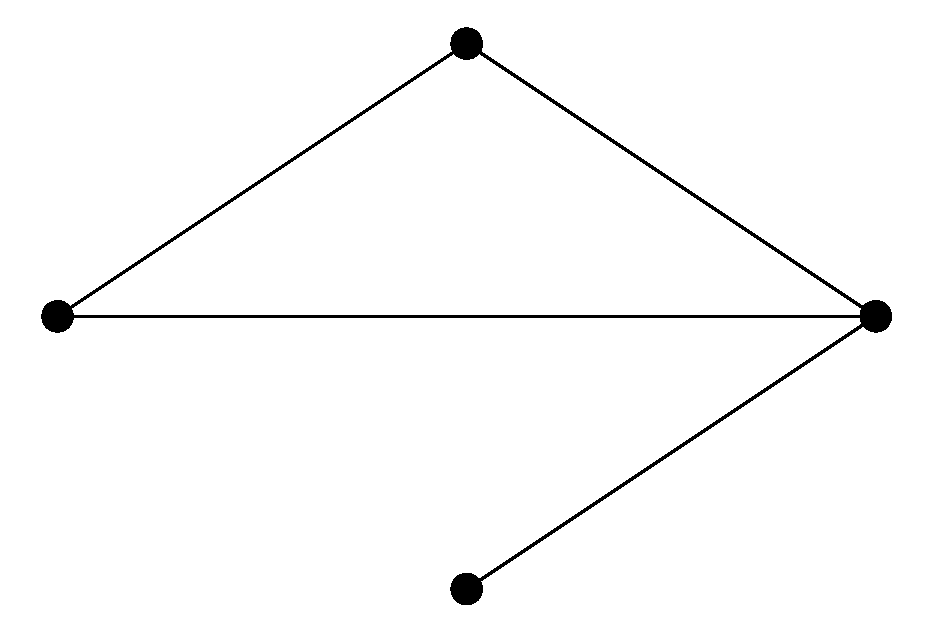
\includegraphics[width=\columnwidth]{images/graph.eps}
         \caption{Grafo casuale.}
     \end{subfigure}
     \hspace{0.8em}
     \begin{subfigure}[t]{3cm}
         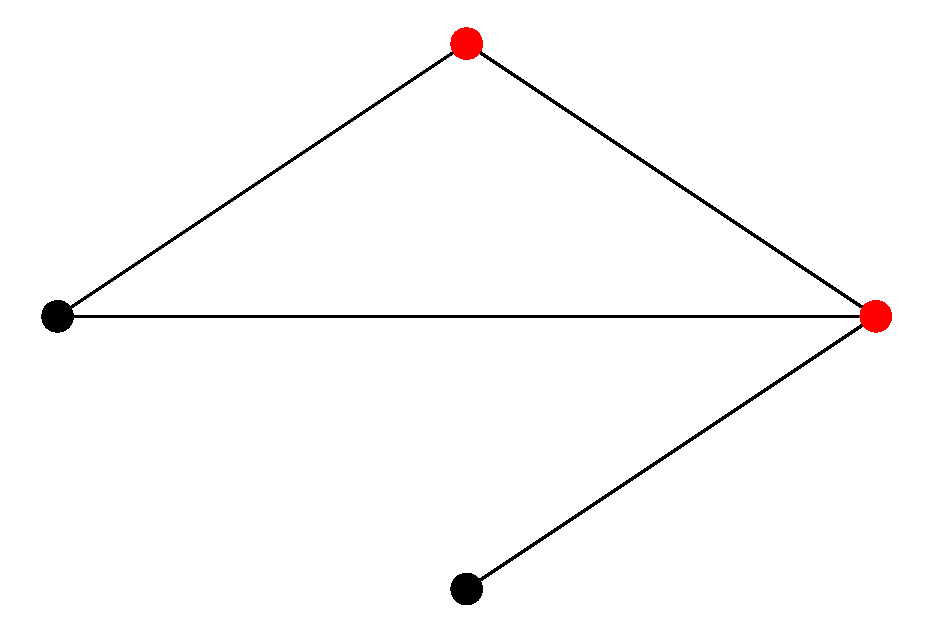
\includegraphics[width=\columnwidth]{images/vc.eps}
         \caption{Vertex cover (in rosso).}
     \end{subfigure}
\end{figure}
Il problema di ottimizzazione del vertex cover minimo consiste nel trovare l'insieme di copertura dei vertici di cardinalità minima. 
\begin{align*}
V_{min}' \, = \, \arg\min_{\tau} \, V' \qquad \mbox{con } \tau= |V'|
\end{align*} 
\end{frame}


\begin{frame}{Generazioni di grafi casuali}
In questo lavoro sono stati utilizzati quattro diversi modelli di generazione di grafi casuali:
\vfill
\begin{itemize}
\item modello di Erdős–Rényi (\textit{percolation})
\vfill
\item modello di Steger-Wormald (\textit{pairing})
\vfill
\item modello di Watts-Strogatz (\textit{rewiring})
\vfill
\item modello di Barabási-Albert (\textit{growth})
\end{itemize}
\vfill
\end{frame}

\renewcommand{\raggedright}{\leftskip=0pt \rightskip=0pt plus 0cm}

\begin{frame}{Modellazione algebrica}
Le diverse fasi in cui si è articolata la modellazione algebrica del problema di ottimizzazione sono state:
\begin{itemize}
\item individuazione degli insiemi
\item individuazione dei parametri
\item individuazione delle variabili
\item definizione dei vincoli e della funzione obiettivo
\end{itemize}
\vfill
Il modello risultante dalla modellazione algebrica del problema risulta quindi essere
\begin{align*}
	\begin{array}{l}
      min\, (\sum_{v \in V} x_v)\\
      x_u + x_v \geq 1  \qquad \forall (u,v) \in E,  u \in V, v \in V \\
      x_v \in {0,1}  \qquad \forall v \in V 
    \end{array}
\end{align*} 
\end{frame}

\begin{frame}{Risultati sperimentali - 1}
\textbf{Grafi di Erdős–Rényi}\\
\parbox{\linewidth}{È possibile notare una correlazione di tipo esponenziale con tra complessità associata al problema ed entrambi i parametri di generazione.}
\vspace{-1cm}
\begin{figure}[h!]
     \centering
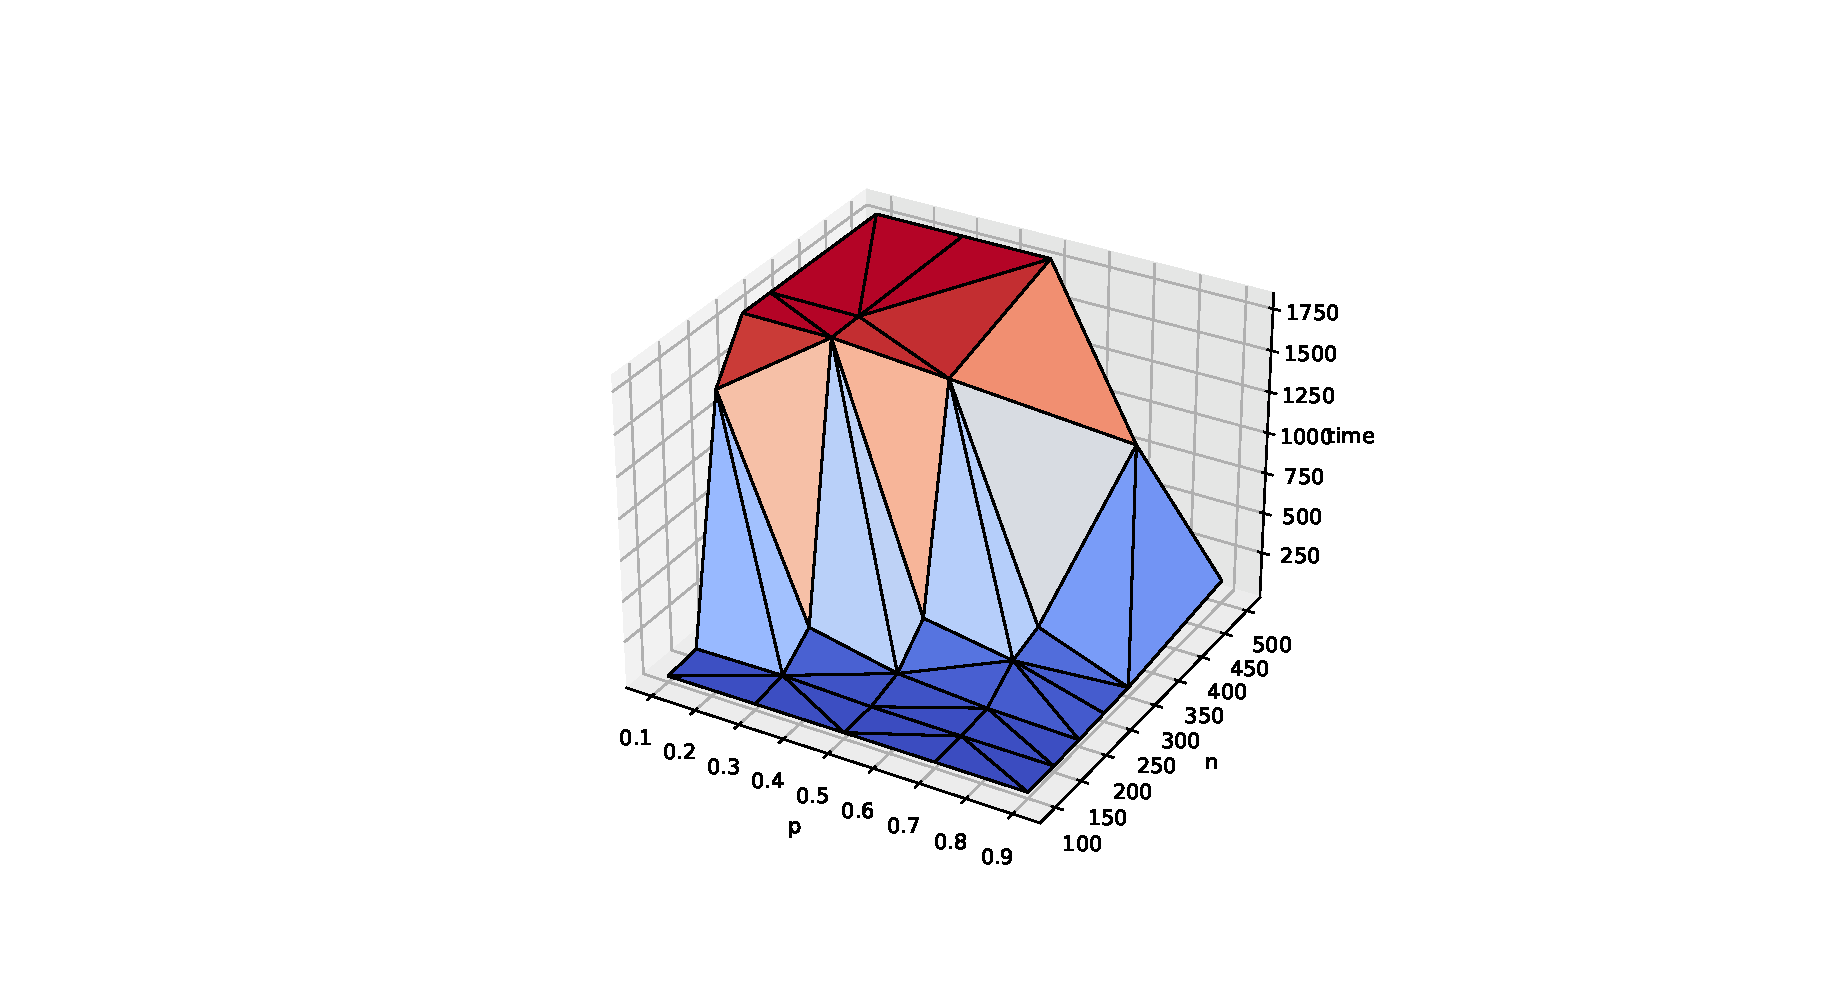
\includegraphics[scale=0.35]{images/gnp-3d.eps}
\vspace{-0.5cm}
\caption{Risultati sperimentali per grafi generati mediante il modello di Erdős–Rényi.}
\end{figure}
\end{frame}

\begin{frame}{Risultati sperimentali - 2}
\textbf{Grafi di Steger-Wormald}\\
\parbox{\linewidth}{In questo caso, una correlazione tra complessità di risoluzione del problema e parametri di generazione non è evidente.}
\begin{figure}[h!]
     \centering
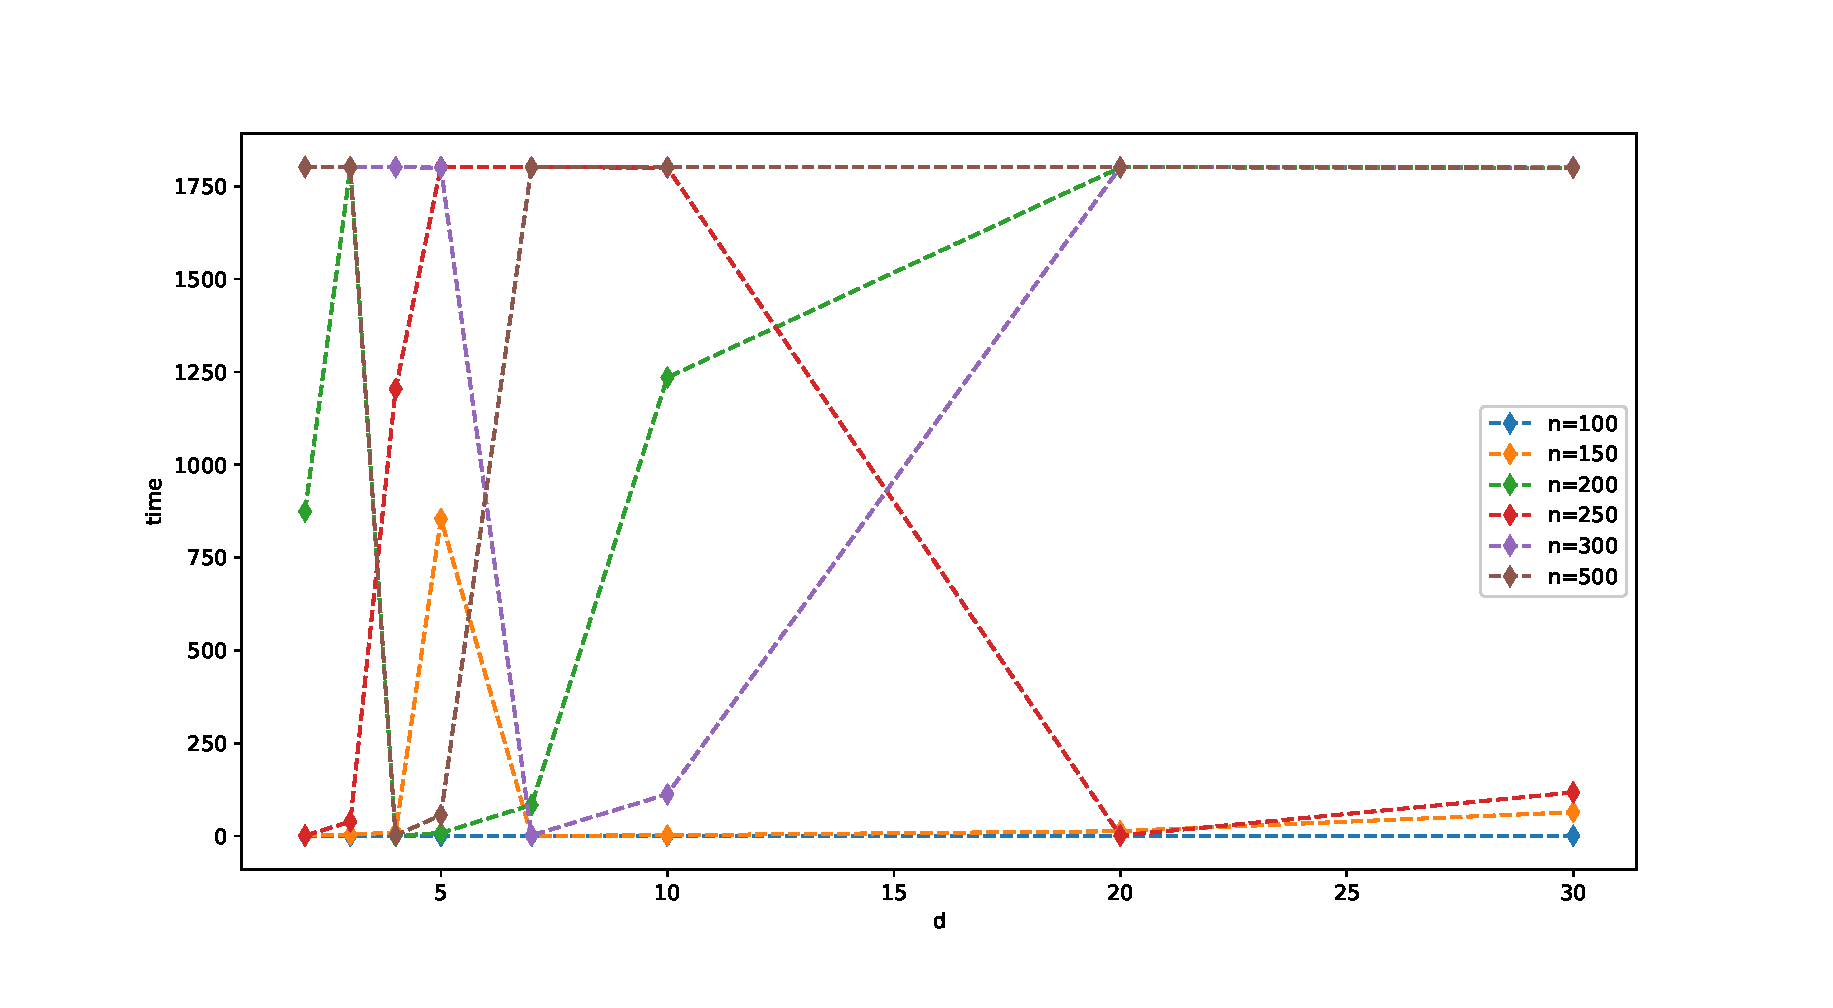
\includegraphics[scale=0.32]{images/rrg-d.eps}
\vspace{-0.1cm}
\caption{Risultati sperimentali per grafi generati mediante il modello di Steger-Wormald.}
\end{figure}
\end{frame}

\begin{frame}{Risultati sperimentali - 3}
\textbf{Grafi di Watts-Strogatz}\\
\parbox{\linewidth}{In questo caso, una correlazione tra complessità di risoluzione del problema e parametri di generazione risulta essere parzialmente definita.}
\begin{figure}[h!]
     \centering
       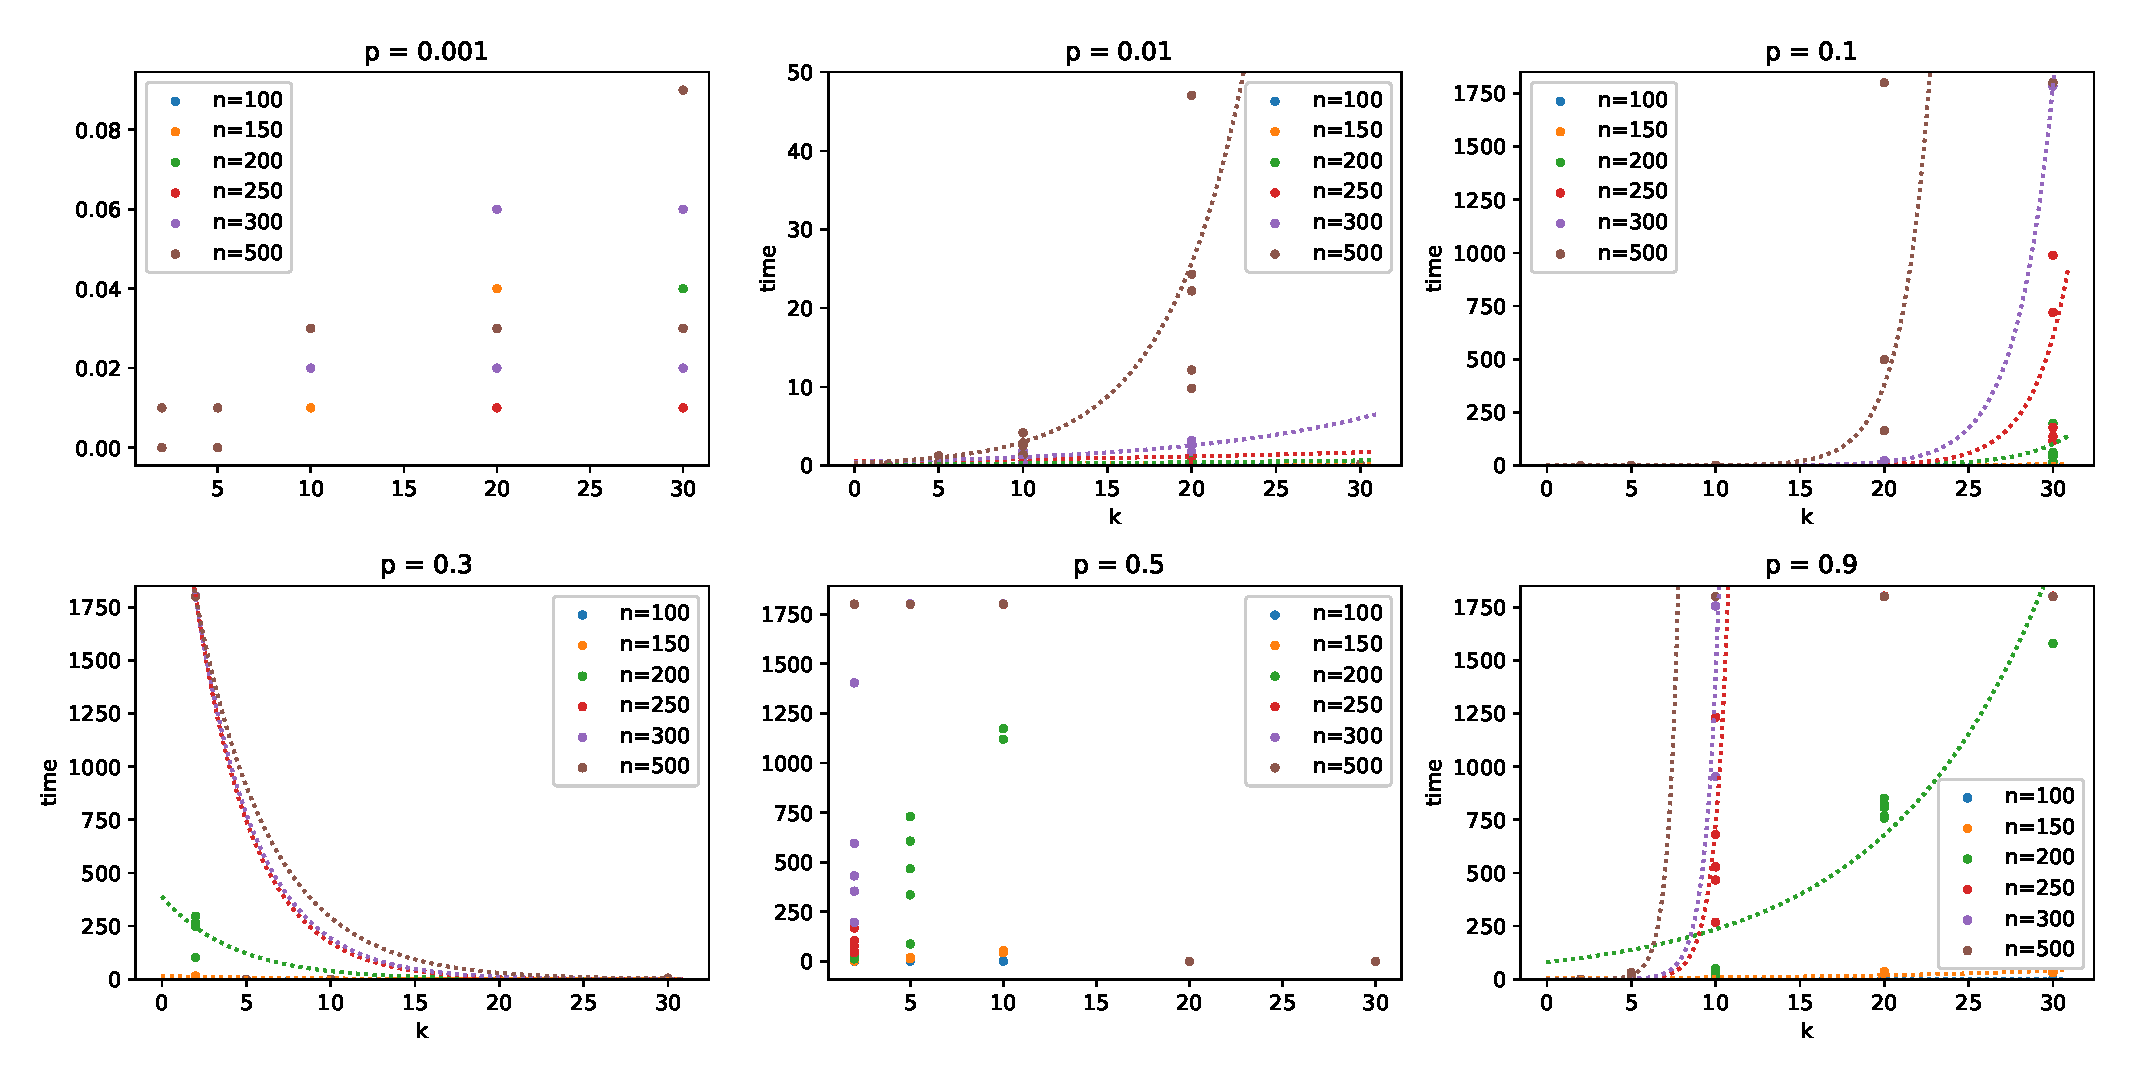
\includegraphics[scale=0.28]{images/wsgp.eps}
       \vspace{-0.1cm}
       \caption{Risultati sperimentali per grafi generati mediante il modello di Watts-Strogatz.}
        \label{fig:wsgp}
\end{figure}
\end{frame}

\begin{frame}{Risultati sperimentali - 4}
\textbf{Grafi di Barabási-Albert}\\
\parbox{\linewidth}{È possibile anche in questo caso notare una correlazione di tipo esponenziale con tra complessità associata al problema ed entrambi i parametri di generazione.}
\vspace*{-1.5cm}
\begin{figure}
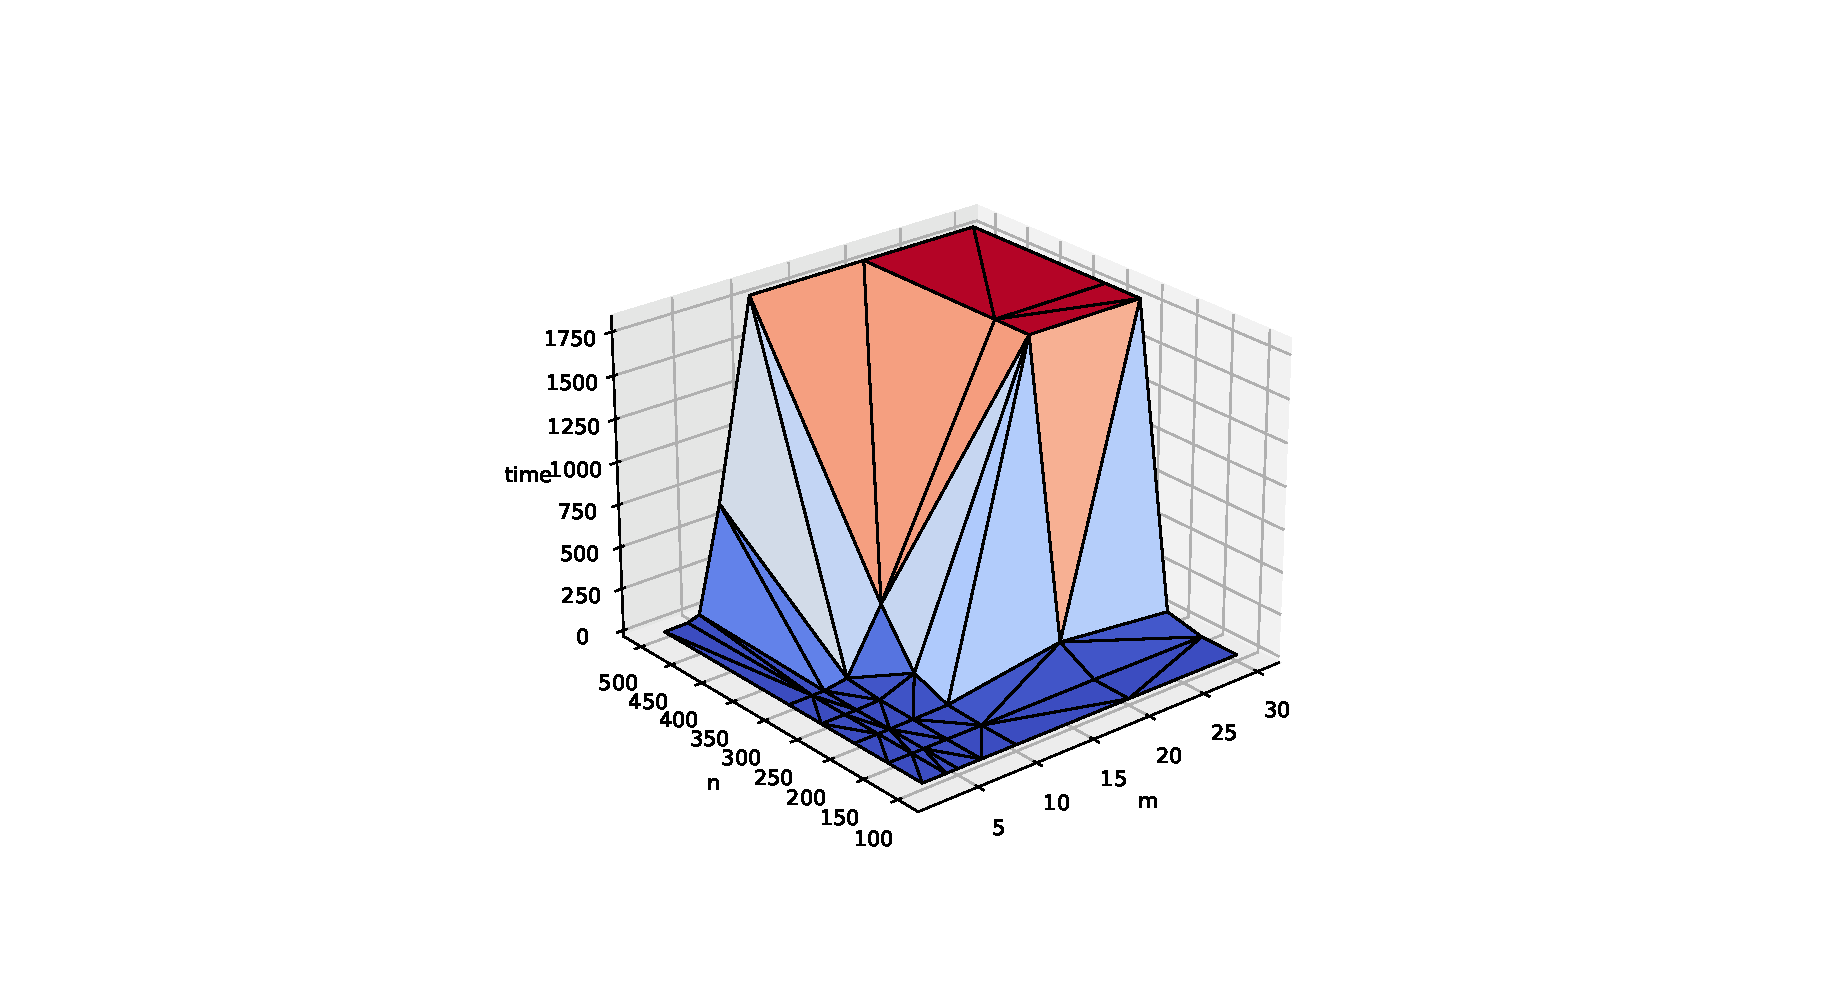
\includegraphics[scale=0.4]{images/bag-3d.eps}
\vspace*{-1.5cm}
\caption{Risultati sperimentali per grafi generati mediante il modello di Barabási-Albert.}
\end{figure}
\end{frame}


\begin{frame}{Conclusioni}
\textbf{Risultati}\\

\begin{itemize}
\item Barabási-Albert e di Erdős–Rényi: correlazione tra complessità di risoluzione e parametri di generazione dei grafi chiaro e coerente
\item Watts-Strogatz: correlazione tra andamento della complessità di risoluzione e parametri di generazione individuata solo parzialmente
\item Steger-Wormald: nessuna correlazione tra parametri di generazione ed andamento della complessità di risoluzione individuata
\end{itemize}

\vfill

\textbf{Possibili futuri sviluppi}\\
\begin{itemize}
\item estensione dell'insieme di combinazioni di parametri utilizzati
\item estensione del time limit imposto al risolutore CPLEX 
\end{itemize}
\end{frame}

\begin{frame}{Ringraziamenti}
\centering
\LARGE Grazie per l'attenzione!
\end{frame}

\begin{frame}
	\maketitle
\end{frame}

\end{document}
